% ===================================================================
%  Week 7 — Morphological Image Processing
% ===================================================================
\documentclass[10pt,aspectratio=169]{beamer}
% ===================================================================
%  Shared Beamer preamble for "Practical Image Processing"
%  English slides. Compile with pdfLaTeX.
% ===================================================================

\usetheme{metropolis}
\usepackage[T1]{fontenc}
\usepackage[utf8]{inputenc}
\usepackage{lmodern}
\usepackage{listings}
\usepackage{tcolorbox}
\usepackage{fontawesome5}
\usepackage{booktabs}
\usepackage{amsmath,amssymb}
\usepackage{tikz}
\usepackage{pgfplots}
\pgfplotsset{compat=1.17}
\usetikzlibrary{arrows.meta,positioning,shapes.geometric,fit,backgrounds,matrix}
\tcbuselibrary{skins,breakable}

% ---- Palette --------------------------------------------------------
\definecolor{coursePrimary}{HTML}{1B4965}   % deep blue
\definecolor{courseAccent}{HTML}{E76F51}    % coral
\definecolor{courseGood}{HTML}{2A9D8F}      % teal
\definecolor{courseBad}{HTML}{C0392B}       % red
\definecolor{courseInfo}{HTML}{2980B9}      % blue
\definecolor{codeBg}{HTML}{F5F6FA}
\definecolor{codeKw}{HTML}{8E44AD}
\definecolor{codeStr}{HTML}{2A9D8F}
\definecolor{codeCom}{HTML}{7F8C8D}

\setbeamercolor{frametitle}{bg=coursePrimary}
\setbeamercolor{progress bar}{fg=courseAccent}
\setbeamercolor{alerted text}{fg=courseAccent}
\metroset{block=fill,sectionpage=progressbar,numbering=fraction}

% ---- Code listings (Python is built into listings) -----------------
\lstdefinestyle{course}{
  backgroundcolor=\color{codeBg},
  basicstyle=\ttfamily\scriptsize,
  keywordstyle=\color{codeKw}\bfseries,
  stringstyle=\color{codeStr},
  commentstyle=\color{codeCom}\itshape,
  numberstyle=\tiny\color{codeCom},
  numbers=left, numbersep=6pt,
  showstringspaces=false, breaklines=true, breakatwhitespace=true,
  tabsize=4, columns=fullflexible,
  frame=single, framesep=4pt, rulecolor=\color{gray!30},
  keepspaces=true, upquote=true, language=Python,
}
\lstset{style=course}
\lstdefinelanguage{bash}{
  keywords={cd,pip,python,venv,source,import}, sensitive=true,
  morecomment=[l]{\#}, morestring=[b]', morestring=[b]",
}

% ---- Reusable callout boxes ----------------------------------------
\newtcolorbox{goodbox}[1][Good practice]{colback=courseGood!8,colframe=courseGood,
  fonttitle=\bfseries,title={\faCheck~#1},boxrule=0.6pt,left=4pt,right=4pt,top=3pt,bottom=3pt}
\newtcolorbox{badbox}[1][Pitfall]{colback=courseBad!8,colframe=courseBad,
  fonttitle=\bfseries,title={\faTimes~#1},boxrule=0.6pt,left=4pt,right=4pt,top=3pt,bottom=3pt}
\newtcolorbox{infobox}[1][Note]{colback=courseInfo!8,colframe=courseInfo,
  fonttitle=\bfseries,title={\faInfoCircle~#1},boxrule=0.6pt,left=4pt,right=4pt,top=3pt,bottom=3pt}
\newtcolorbox{mathbox}[1][Math]{colback=coursePrimary!6,colframe=coursePrimary,
  fonttitle=\bfseries,title={\faCalculator~#1},boxrule=0.6pt,left=4pt,right=4pt,top=3pt,bottom=3pt}

\newcommand{\keyidea}[1]{\begin{alertblock}{Key idea}#1\end{alertblock}}
\newcommand{\term}[1]{\textbf{\color{coursePrimary}#1}}
\newcommand{\code}[1]{\lstinline[basicstyle=\ttfamily\small]|#1|}

% ---- A helper to draw a small pixel grid, cells shaded by value ----
% \pixelgrid{ {10,20,120,200,240}, {30,60,130,180,230}, ... }
\newcommand{\pixelgrid}[1]{%
  \begin{tikzpicture}[font=\scriptsize,scale=0.6]
    \foreach \row [count=\ry] in {#1} {
      \foreach \val [count=\cx] in \row {
        \draw[gray,fill=coursePrimary!8] (\cx,-\ry) rectangle ++(1,-1);
        \node at (\cx+0.5,-\ry-0.5) {\val};
      }
    }
  \end{tikzpicture}}


\title{Morphological Processing}
\subtitle{Week 7 — Shaping binary images}
\author{Practical Image Processing}
\date{Lecture 7 \textbullet\ 60--70 min}

\begin{document}

\maketitle

\begin{frame}{Recap \& today}
  \begin{columns}[T]
    \begin{column}{0.58\textwidth}
      \begin{itemize}
        \item Wk2/8: thresholding gives a \term{binary} image — but it's messy (specks, gaps).
        \item \alert{Today:} \term{morphology} — operations that grow, shrink, and clean binary
              shapes using a \term{structuring element}.
      \end{itemize}
    \end{column}
    \begin{column}{0.42\textwidth}
      \begin{alertblock}{DocScan milestone}
        After thresholding the digits, morphology removes noise and fills gaps so each digit is
        a clean, separable blob.
      \end{alertblock}
    \end{column}
  \end{columns}
\end{frame}

\begin{frame}{Roadmap}\tableofcontents\end{frame}

% ==================================================================
\section{The two basic operations}
% ==================================================================

\begin{frame}{The structuring element}
  \begin{itemize}
    \item A small shape (the \term{SE} / kernel) that slides over the binary image — like a probe.
    \item Common shapes: rectangle, ellipse, cross. Its \term{size} sets how aggressive the effect is.
    \item Morphology asks: does the SE \emph{fit} (erosion) or \emph{hit} (dilation) the shape here?
  \end{itemize}
  \begin{mathbox}
    \code{cv2.getStructuringElement(cv2.MORPH\_ELLIPSE, (3,3))} — a $3\times3$ elliptical probe.
  \end{mathbox}
\end{frame}

\begin{frame}{Erosion \& dilation — on real digits}
  \begin{columns}[T]
    \begin{column}{0.33\textwidth}\begin{center}
      
\includegraphics[width=\linewidth]{../assets/binary.png}\\{\scriptsize binary digits}
    \end{center}\end{column}
    \begin{column}{0.33\textwidth}\begin{center}
      
\includegraphics[width=\linewidth]{../assets/erode.png}\\{\scriptsize erosion (thinner)}
    \end{center}\end{column}
    \begin{column}{0.33\textwidth}\begin{center}
      
\includegraphics[width=\linewidth]{../assets/dilate.png}\\{\scriptsize dilation (thicker)}
    \end{center}\end{column}
  \end{columns}
  \vspace{3pt}
  \begin{itemize}
    \item \term{Erosion}: keep a pixel only if the SE fits entirely inside the shape $\rightarrow$ shrinks, removes thin bits.
    \item \term{Dilation}: set a pixel if the SE touches the shape $\rightarrow$ grows, fills small holes.
  \end{itemize}
\end{frame}

\begin{frame}{Erosion and dilation are duals}
  \begin{itemize}
    \item Dilating the foreground = eroding the background (and vice versa).
    \item Erosion removes: thin protrusions, small objects, and it \term{separates} touching objects.
    \item Dilation adds: fills gaps, connects nearby pieces, and \term{thickens} thin strokes.
  \end{itemize}
  \begin{badbox}
    Each also distorts: erosion can break a thin digit; dilation can merge two close digits. Size matters.
  \end{badbox}
\end{frame}

% ==================================================================
\section{Opening \& closing}
% ==================================================================

\begin{frame}{Opening = erode then dilate}
  \begin{columns}[T]
    \begin{column}{0.5\textwidth}\begin{center}
      
\includegraphics[width=0.95\linewidth]{../assets/noisy.png}\\{\scriptsize binary + speckles}\\[4pt]
      
\includegraphics[width=0.95\linewidth]{../assets/open.png}\\{\scriptsize opening: specks gone}
    \end{center}\end{column}
    \begin{column}{0.5\textwidth}
      \begin{itemize}
        \item \term{Opening} removes small bright specks while keeping the digits' size (erode kills them, dilate restores the rest).
        \item The classic ``clean up salt noise on a binary mask'' operation.
      \end{itemize}
    \end{column}
  \end{columns}
\end{frame}

\begin{frame}{Closing = dilate then erode}
  \begin{columns}[T]
    \begin{column}{0.5\textwidth}\begin{center}
      
\includegraphics[width=0.95\linewidth]{../assets/binary.png}\\{\scriptsize binary}\\[4pt]
      
\includegraphics[width=0.95\linewidth]{../assets/close.png}\\{\scriptsize closing: gaps filled}
    \end{center}\end{column}
    \begin{column}{0.5\textwidth}
      \begin{itemize}
        \item \term{Closing} fills small holes and gaps inside shapes while keeping the size.
        \item Repairs a digit broken by thresholding into a solid stroke.
      \end{itemize}
    \end{column}
  \end{columns}
\end{frame}

\begin{frame}{Opening vs closing: remember the effect}
  \begin{center}
  \begin{tabular}{@{}lll@{}}
    \toprule
    \textbf{Operation} & \textbf{Order} & \textbf{Effect} \\
    \midrule
    Opening & erode $\rightarrow$ dilate & removes small \emph{bright} specks, breaks thin links \\
    Closing & dilate $\rightarrow$ erode & fills small \emph{dark} holes, bridges gaps \\
    \bottomrule
  \end{tabular}
  \end{center}
  \keyidea{Opening cleans the outside; closing repairs the inside. Both keep the overall size, unlike raw erosion/dilation.}
\end{frame}

% ==================================================================
\section{More operations}
% ==================================================================

\begin{frame}{Morphological gradient, top-hat, black-hat}
  \begin{columns}[T]
    \begin{column}{0.4\textwidth}\begin{center}
      
\includegraphics[width=\linewidth]{../assets/gradient.png}\\{\scriptsize gradient = outline}
    \end{center}\end{column}
    \begin{column}{0.6\textwidth}
      \begin{itemize}
        \item \term{Gradient} = dilation $-$ erosion $\rightarrow$ the object outline.
        \item \term{Top-hat} = image $-$ opening $\rightarrow$ small bright details (uneven lighting correction!).
        \item \term{Black-hat} = closing $-$ image $\rightarrow$ small dark details.
      \end{itemize}
    \end{column}
  \end{columns}
  \vspace{3pt}
  \begin{goodbox}
    Top-hat is a lighting fix: it isolates the digits from a slowly-varying background.
  \end{goodbox}
\end{frame}

\begin{frame}{Grayscale morphology (brief)}
  \begin{itemize}
    \item Morphology also works on grayscale: erosion = local min, dilation = local max.
    \item Top-hat on grayscale removes a smooth background gradient — great before thresholding.
    \item So morphology isn't only for binary — it's a general shape/intensity tool.
  \end{itemize}
\end{frame}

\begin{frame}{Structuring-element shapes}
  \begin{center}
  \begin{tabular}{@{}lll@{}}
    \toprule
    \textbf{Shape} & \textbf{When} & \textbf{Note} \\
    \midrule
    Rectangle & general cleanup & fast, blocky effect \\
    Ellipse & round objects & smoother, more natural \\
    Cross & thin connectors & minimal, gentle \\
    Line (h/v) & directional & remove/keep horizontal or vertical strokes \\
    \bottomrule
  \end{tabular}
  \end{center}
  \keyidea{A line SE can remove table lines while keeping text — the shape of the probe is a design choice.}
\end{frame}

\begin{frame}{Boundary extraction \& hole filling}
  \begin{itemize}
    \item \term{Boundary} = image $-$ erosion (a thin outline; cf.\ the morphological gradient).
    \item \term{Hole filling}: fill enclosed dark regions inside a shape (a solid digit from a hollow one).
    \item These build on erosion/dilation — morphology is a small toolkit that composes into many effects.
  \end{itemize}
\end{frame}

% ==================================================================
\section{In-class exercise}
% ==================================================================

\begin{frame}{\faPen~In-class exercise (12 min)}
  \begin{infobox}[Pick the operation]
  \end{infobox}
  Your thresholded meter has these problems. Which morphology fixes each?
  \begin{enumerate}
    \item Scattered single white pixels (salt) around the digits.
    \item One digit is broken into two pieces by a threshold gap.
    \item Two adjacent digits are touching and need to be separated for counting.
    \item You want just the outline of each digit.
  \end{enumerate}
\end{frame}

\begin{frame}{\faPen~Debrief}
  \begin{itemize}
    \item (1) Salt specks $\rightarrow$ \term{opening} (small SE). (2) Broken digit $\rightarrow$ \term{closing}.
    \item (3) Touching digits $\rightarrow$ \term{erosion} (carefully) to separate, or a watershed (Week 8).
    \item (4) Outline $\rightarrow$ \term{morphological gradient}.
  \end{itemize}
  \keyidea{Diagnose the defect (specks / gaps / merges), then choose the matching operation and SE size.}
\end{frame}

% ==================================================================
\section{Deep dive}
% ==================================================================

\begin{frame}{Structuring element: shape \& size matter}
  \begin{itemize}
    \item A larger SE = a stronger effect (removes bigger specks / fills bigger gaps) but more distortion.
    \item Shape matters: a vertical SE affects vertical strokes differently than a horizontal one.
    \item Rule: use the \emph{smallest} SE that fixes the defect — bigger erases real detail.
  \end{itemize}
  \begin{badbox}
    A too-large SE turns your digits into unrecognizable blobs. Tune the size on real data.
  \end{badbox}
\end{frame}

\begin{frame}{Skeletonization \& thinning}
  \begin{itemize}
    \item \term{Skeleton}: repeatedly thin a shape to a 1-pixel ``spine'' — its topological essence.
    \item Useful for character/stroke analysis and measuring connectivity.
    \item Related: \term{hit-or-miss} finds exact local patterns (corners, endpoints).
  \end{itemize}
\end{frame}

\begin{frame}{A morphology cleanup pipeline}
  \begin{center}
  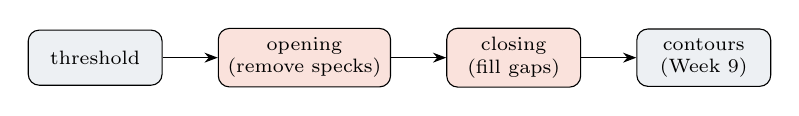
\begin{tikzpicture}[font=\scriptsize,>=Stealth,node distance=3mm and 7mm,
    b/.style={draw,rounded corners,fill=coursePrimary!8,minimum height=7mm,minimum width=17mm,align=center}]
    \node[b] (thr){threshold};
    \node[b,right=of thr,fill=courseAccent!20] (open){opening\\(remove specks)};
    \node[b,right=of open,fill=courseAccent!20] (close){closing\\(fill gaps)};
    \node[b,right=of close] (cc){contours\\(Week 9)};
    \draw[->](thr)--(open);\draw[->](open)--(close);\draw[->](close)--(cc);
  \end{tikzpicture}
  \end{center}
  \begin{itemize}
    \item Typical DocScan order: threshold $\rightarrow$ open (kill noise) $\rightarrow$ close (repair digits) $\rightarrow$ contours.
    \item Order matters: opening before closing avoids fusing a speck into a digit.
  \end{itemize}
\end{frame}

\begin{frame}{Removing lines, keeping text}
  \begin{itemize}
    \item A form has table/underline strokes you want gone but the text kept.
    \item Use a long \emph{horizontal} line SE with opening to isolate horizontal lines, then subtract them.
    \item A directional SE is a precise tool — it operates only on structures of a chosen orientation and length.
  \end{itemize}
  \begin{goodbox}
    For a scanned form (a DocScan case), this cleanly separates rules/boxes from the handwritten content.
  \end{goodbox}
\end{frame}

\begin{frame}{Morphology vs blurring}
  \begin{itemize}
    \item Blurring averages (softens everything); morphology reasons about \emph{shape} (keeps edges hard).
    \item To remove specks from a \emph{binary} mask, opening beats a blur (which would gray it out).
    \item Use blur on grayscale/noise; use morphology on binary shapes.
  \end{itemize}
  \keyidea{Morphology is the right tool once you have a binary mask — it's shape surgery, not smoothing.}
\end{frame}

% ==================================================================
\section{Wrap-up}
% ==================================================================

\begin{frame}{What you should now be able to do}
  \begin{itemize}
    \item Explain erosion/dilation via a structuring element (fit vs hit).
    \item Use opening (remove specks) and closing (fill gaps); pick the SE size.
    \item Apply gradient/top-hat/black-hat; correct uneven lighting with top-hat.
    \item Build a threshold $\rightarrow$ morphology cleanup pipeline for the digits.
  \end{itemize}
\end{frame}

\begin{frame}[fragile]{Morphology in code}
\begin{lstlisting}[language=Python]
k = cv2.getStructuringElement(cv2.MORPH_ELLIPSE, (3, 3))
op  = cv2.morphologyEx(binary, cv2.MORPH_OPEN,  k)   # remove specks
cl  = cv2.morphologyEx(binary, cv2.MORPH_CLOSE, k)   # fill gaps
top = cv2.morphologyEx(gray,   cv2.MORPH_TOPHAT, big_k)  # lighting fix
\end{lstlisting}
  \code{morphologyEx} covers open/close/gradient/top-hat/black-hat with one call.
\end{frame}

\begin{frame}{This week's deliverable}
  \begin{alertblock}{Due before Week 8 (see \code{project/})}
    On a thresholded meter/plate (from Week 2):
    \begin{enumerate}
      \item Demonstrate erosion, dilation, opening, closing; explain each effect.
      \item Use opening to remove speckle noise and closing to repair broken digits.
      \item Apply top-hat to a photo with uneven lighting; compare to before.
      \item DocScan milestone: produce a clean binary where each digit is a solid, separable blob.
    \end{enumerate}
  \end{alertblock}
\end{frame}

\begin{frame}[standout]
  Threshold makes it binary; morphology makes it clean.\\[4pt]
  \normalsize Opening removes specks, closing fills gaps — shape surgery.
\end{frame}

\end{document}
